
\section{Study Design}\label{sec:literature-review-study-design}

\begin{figure}[htp]
\centering
\fbox{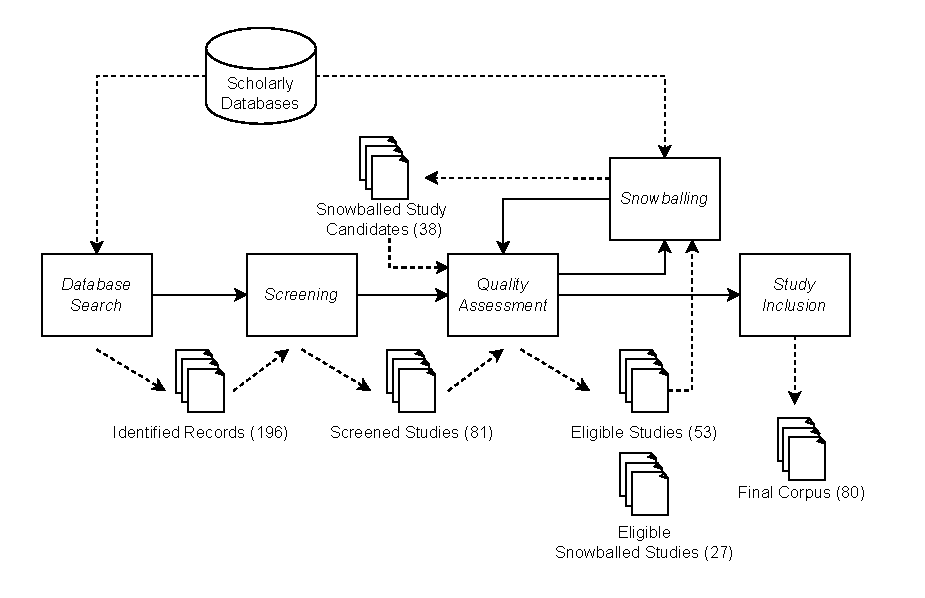
\includegraphics[width=\textwidth]{figures/Literature Review/Study Design Diagram.drawio.pdf}}
\caption{Overview of study design.}
\label{fig:literature_review_study_design_overview}
\end{figure}

This review followed established guidelines for systematic literature reviews~\cite{kitchenham2007guidelines, wohlin2020guidelines} to ensure rigor and reproducibility. A structured search was conducted across Scopus, Web of Science, IEEE Xplore, and the ACM Digital Library using combinations of Digital Twin and System-of-Systems terminology. Core expressions included \textit{“digital twin*” AND “system* of systems”} alongside common variants identified during preliminary exploration (e.g., \textit{“aggregated digital twin*”}, \textit{“system of digital twins”}, and \textit{“digital twin of systems”}). This initial search yielded 317 publications. After duplicate removal and screening titles and abstracts using predefined inclusion and exclusion criteria, 196 studies remained for full-text review. Quality assessment—evaluating clarity of DT and SoS descriptions, tangibility of contributions, and reporting quality—narrowed this set to 53 high-quality primary studies. The overall workflow is summarized in \figref{fig:literature_review_study_design_overview}.

\begin{table*}[]
\centering
\setlength{\tabcolsep}{1em}
\caption{Search statistics}
\label{tab:literature_review_search_statistics}
\footnotesize
\begin{tabular}{@{}lrrr@{\hspace{2pt}}lr@{}}
\toprule
\multicolumn{1}{c}{\textbf{Search round}} & \multicolumn{1}{c}{\textbf{All}} & \multicolumn{1}{c}{\textbf{Excluded}} & \multicolumn{2}{c}{\textbf{Included}} & \multicolumn{1}{c}{\textbf{Agreement}} \\ \midrule
\textbf{Automated search} & & & & & \\
\;\;\corner{} Duplicate removal & 317 & 121 & 196 &   &  \\
\;\;\corner{} E0 & 196 & 71 & 125 &   &  \\
\;\;\corner{} E1--E3 & 125 & 44 & \textbf{81} & & $IRA=0.88$ / $\kappa=0.734$ \\
\textbf{Quality assessment} & & & & & \\
\;\;\corner{} Q1 or Q2 insufficient & 81 & 22 & 59 &   &  \\
\;\;\corner{} Q3 insufficient & 59 & 6 & 53 &   &  \\
\;\;\corner{} Q4 insufficient & 53 & 0 & 53 &   &  \\
\textbf{Subtotal} & \textbf{317} & \textbf{264} & \included{53} & \textbf{(16.72\%)} & \\
\midrule
\textbf{Snowballing} & & & & & \\
\;\;\corner{} Backward & & & & & \\
\;\;\;\;\corner{} Selection by reference & 1\,666 & 1\,521 & 145 & & \\
\;\;\;\;\corner{} Selection by abstract & 145 & 132 & \textbf{13} & & \\
\;\;\corner{} Forward & 586 & 561 & \textbf{25} & &  \\
\;\;\corner{} Total abstracts screened & 731 & 693  & \textbf{38} & & $IRA=0.944$ / $\kappa=0.488$ \\
\textbf{Quality assessment} & & & & & \\
\;\;\corner{} Q1 or Q2 insufficient & 38 & 9 & 29 &   &  \\
\;\;\corner{} Q3 insufficient & 29 & 2 & 27 &   &  \\
\;\;\corner{} Q4 insufficient & 27 & 0 & \textbf{27} &  &  \\
\textbf{Subtotal} & \textbf{2\,252} & \textbf{2\,225} & \included{27} & \textbf{(1.19\%)} & \\
\midrule
\textbf{Total} & \textbf{2\,569} & \textbf{2\,489} & \included{80} & \textbf{(3.11\%)} & \\
\bottomrule
\end{tabular}
\end{table*}

To broaden coverage, forward and backward snowballing was performed following \citet{wohlin2020guidelines}, applying the same screening and quality criteria to referenced and citing works. This process added 27 additional studies, producing a final set of \textbf{80 primary papers}. Screening was conducted by two reviewers, with disagreements resolved through discussion, and \tabref{tab:literature_review_search_statistics} summarizes the search and screening outcomes.

Data extraction followed a structured coding process addressing conceptual alignment, architectural and modelling practices, treatment of non-functional properties, research maturity, and implementation choices. Synthesis combined quantitative and qualitative techniques~\cite{franzosi2010quantitative, rodgers2009testing} and was guided by established SoS~\cite{nielsen2015systems}, DT~\cite{kritzinger2018digital, david2024infonomics}, and dependability~\cite{avizienis2004basic} taxonomies. All extraction scripts and aggregated datasets are available in the replication package.% \footnote{\url{https://github.com/ssm-lab/system-of-twinned-systems-replication-package}}
\footnote{\url{https://zenodo.org/records/18891164}}